\documentclass{article}
\usepackage[a4paper, total={6in, 8in}]{geometry}
\usepackage{cite}
\usepackage{titlesec}
\usepackage{amsmath}
\usepackage{caption}
\usepackage{graphicx}
\usepackage{float}
\setcounter{secnumdepth}{4}
\graphicspath{{./figures/}}
\allowdisplaybreaks
\title{Data Analysis for Predictive Maintenance of a Straightening Machine in the Steel Industry}
\date{2023-XX-XX}
\author{Paul Barron}
\begin{document}
\pagenumbering{gobble}
\maketitle
\newpage
\pagenumbering{arabic}
\tableofcontents
\newpage
\section{Abstract}
Large large machinery is expensive to run and downtime can be very costly. There is a large area of work dedicated to analyzing the health of a machine, predicting the remaining life and time to failure.
\newpage
\section{Introduction}
The aims of this project are to:
\begin{itemize}
\item Understand what signals are related to each other
\item Understand signals from a statistical point of view
\item Identify which features are the important ones and which are not of interest
\end{itemize}
\clearpage  
\section{Literature Review}
\subsection{Condition Monitoring}
Reference ~\cite{caesarendra2017review}.\\
Reference ~\cite{james2013introduction}.\\
Reference ~\cite{soualhi2021novel}.
"We tend to select statistical learning methods on the basis of whether
the response is quantitative or qualitative; i.e. we might use linear regression when quantitative and logistic regression when qualitative." From textbook.
\subsection{Bearing Vibration Analysis?}
\subsection{Straightening Machine}
\clearpage 
\section{Methodology}
Preprocessing: you could standardize the signals, eliminate the dc-offset, … before calculating the features.
Calculate features of the different signals, i.e., correlations between raw signals, kurtosis, mean, skewness, …,
Verify features which are extracted from the diagnostic feature extraction toolbox, i.e., what it is kurtosis, THD,… for the toolbox. You can compare the results given by the matlab function and the toolbox. Important to look at the formula which is given on the help description of the function.

Compute correlations between 2 features.
Calculate a in X1 = aX2, where X1 and X2 represents the features.
Calculate R2, which relates to the variance in linear regression models.
Plot some of the regression models between 2 features which are highly correlated where X1 is one axis, and X2 is the other axis. Do not plot all of them.

Compute a multivariable regression model.
Guide yourself by eliminating features which are highly correlated between each other by using the info you got in the previous part where you compute correlations between 2 features.

\subsection{Description of Data}
The data used for this analysis consists of an hour of operational data for 15 days. I do now know whether it was taken from the same time each day. The assumption is that the file name corresponds with the data that the data was taken.
The file names are given in \ref{fileNames}.
\begin{center}
\begin{tabular}{ |l| } 
 \hline
 B\_30\_03.mat \\
 \hline 
 B\_31\_03.mat \\
 \hline 
 B\_01\_04.mat \\
 \hline 
 B\_02\_04.mat \\
 \hline
 B\_03\_04.mat \\
 \hline 
 B\_04\_04.mat \\
 \hline 
 B\_05\_04.mat \\
 \hline
 B\_06\_04.mat \\
 \hline 
 B\_07\_04.mat \\
 \hline 
 B\_08\_04.mat \\
 \hline 
 B\_09\_04.mat \\
 \hline 
 B\_10\_04.mat \\
 \hline
 B\_11\_04.mat \\
 \hline 
 B\_12\_04.mat \\
 \hline
 B\_13\_04.mat \\
 \hline
\end{tabular}
\captionof{table}{File names which indicate the day the data was taken}\label{fileNames}
\end{center}

The list of signals given be the company are given in Table \ref{signalNames}.
\begin{center}
\begin{tabular}{ |c|l| }
 \hline
 Signal Number & Signal Name \\ 
 \hline
21:07 & Angle over Rolls (deg) \\
 \hline
21:10 & Position over Rolls (mm) \\
 \hline
21:12 & Actual moment over Rolls (Nm) \\
 \hline
21:17 & Angle under roll (deg) \\
 \hline
21:20 & Actual moment under Rolls (Nm) \\
 \hline
21:28 & Vibration measurements (mm/s) \\ 
 \hline              
21:31 & Width position (mm) \\
 \hline
21:32 & Height position (mm) \\
 \hline
21:33 & Error position for height (mm) \\
 \hline
21:34 & Error position for the width (mm) \\
 \hline
21:35 & Set point force (kN) \\
 \hline
21:36 & Actual force (kN) \\
 \hline
\end{tabular}
\captionof{table}{Signal Names}\label{signalNames}
\end{center}

Figure \ref{fig:SignalTrace21.20} shows 21:20 Actual moment under Rolls (Nm)
\begin{figure}[H]
    \centering
    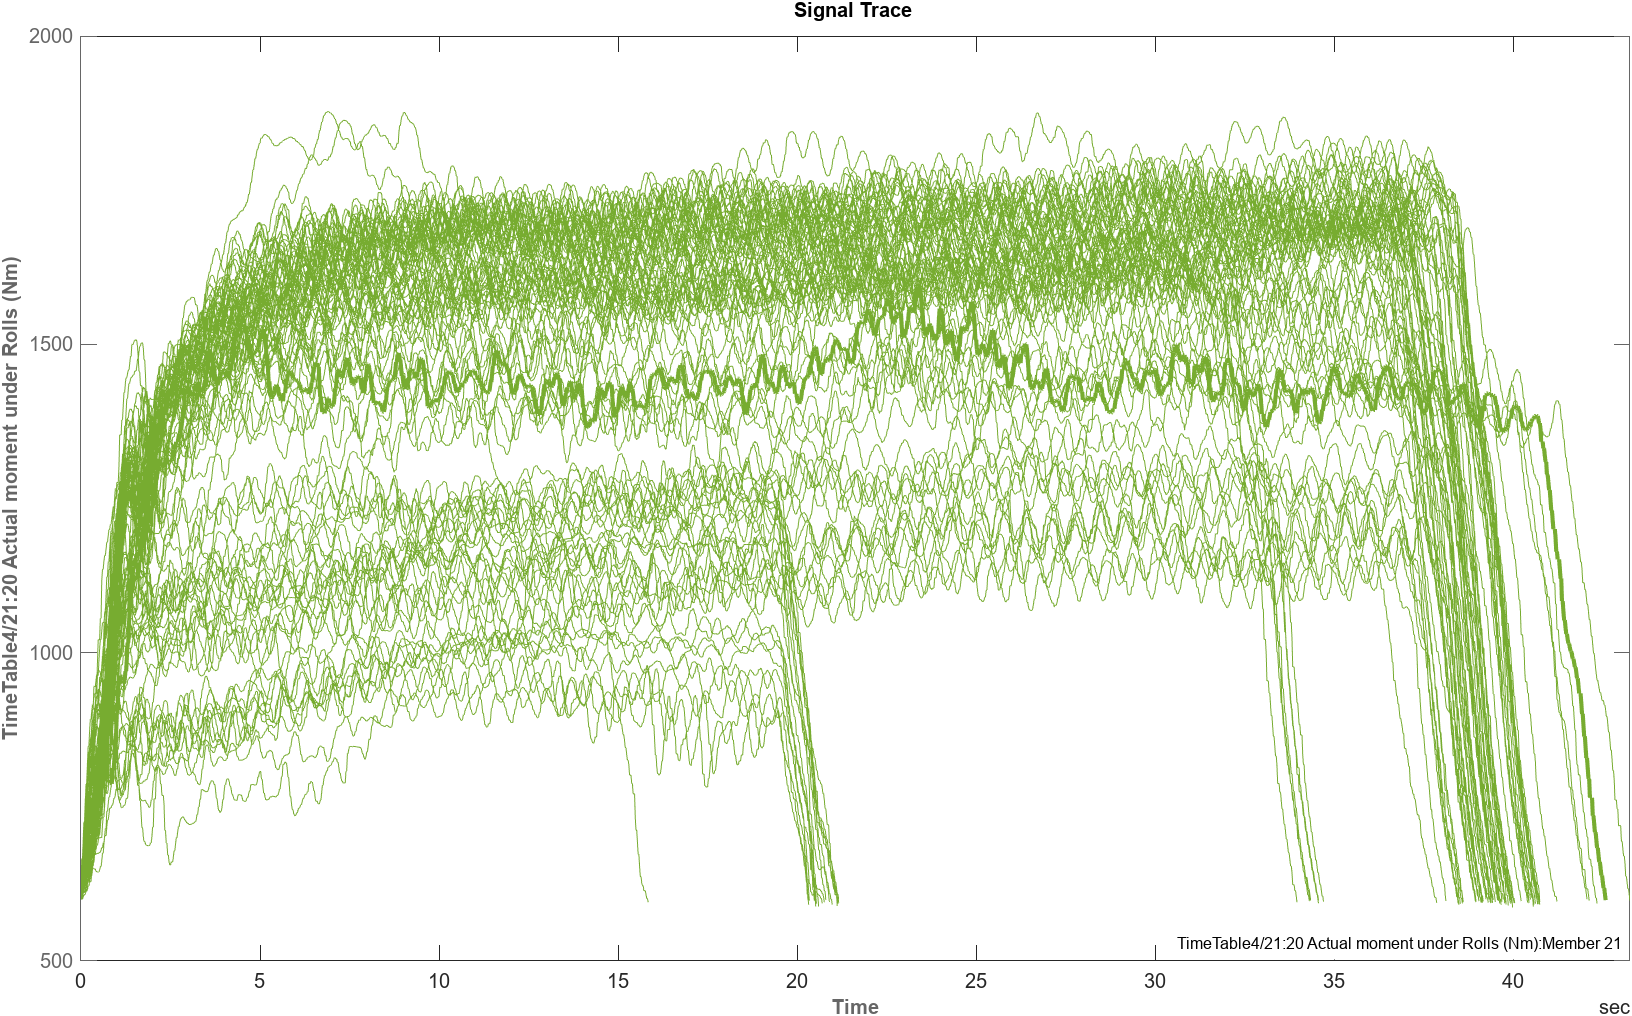
\includegraphics[width=\textwidth, height=\textheight, keepaspectratio]{figures/SignalTrace21.20.png}
    \caption{Signal Trace 21.20}
    \label{fig:SignalTrace21.20}
\end{figure}

Figure \ref{fig:SignalTrace21.12} shows ...
\begin{figure}[H]
    \centering
    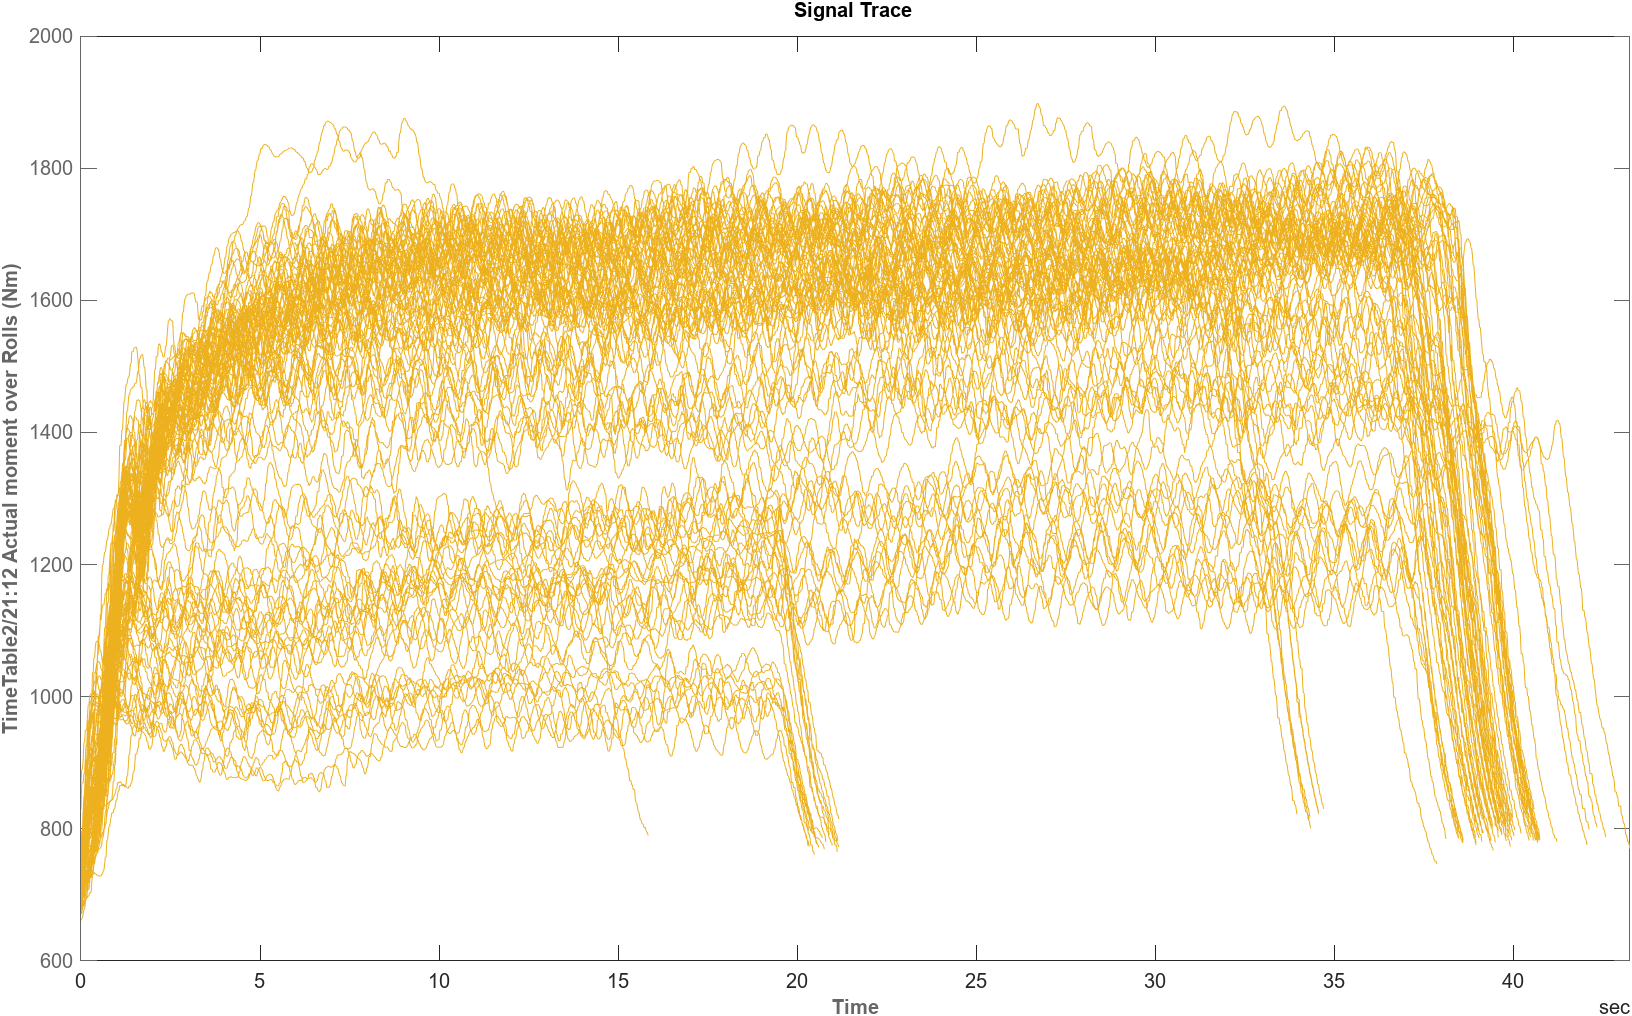
\includegraphics[width=\textwidth, height=\textheight, keepaspectratio]{figures/SignalTrace21.12.png}
    \caption{Signal Trace 21.12}
    \label{fig:SignalTrace21.12}
\end{figure}

Figure \ref{fig:SignalTrace21.28} shows ...
\begin{figure}[H]
    \centering
    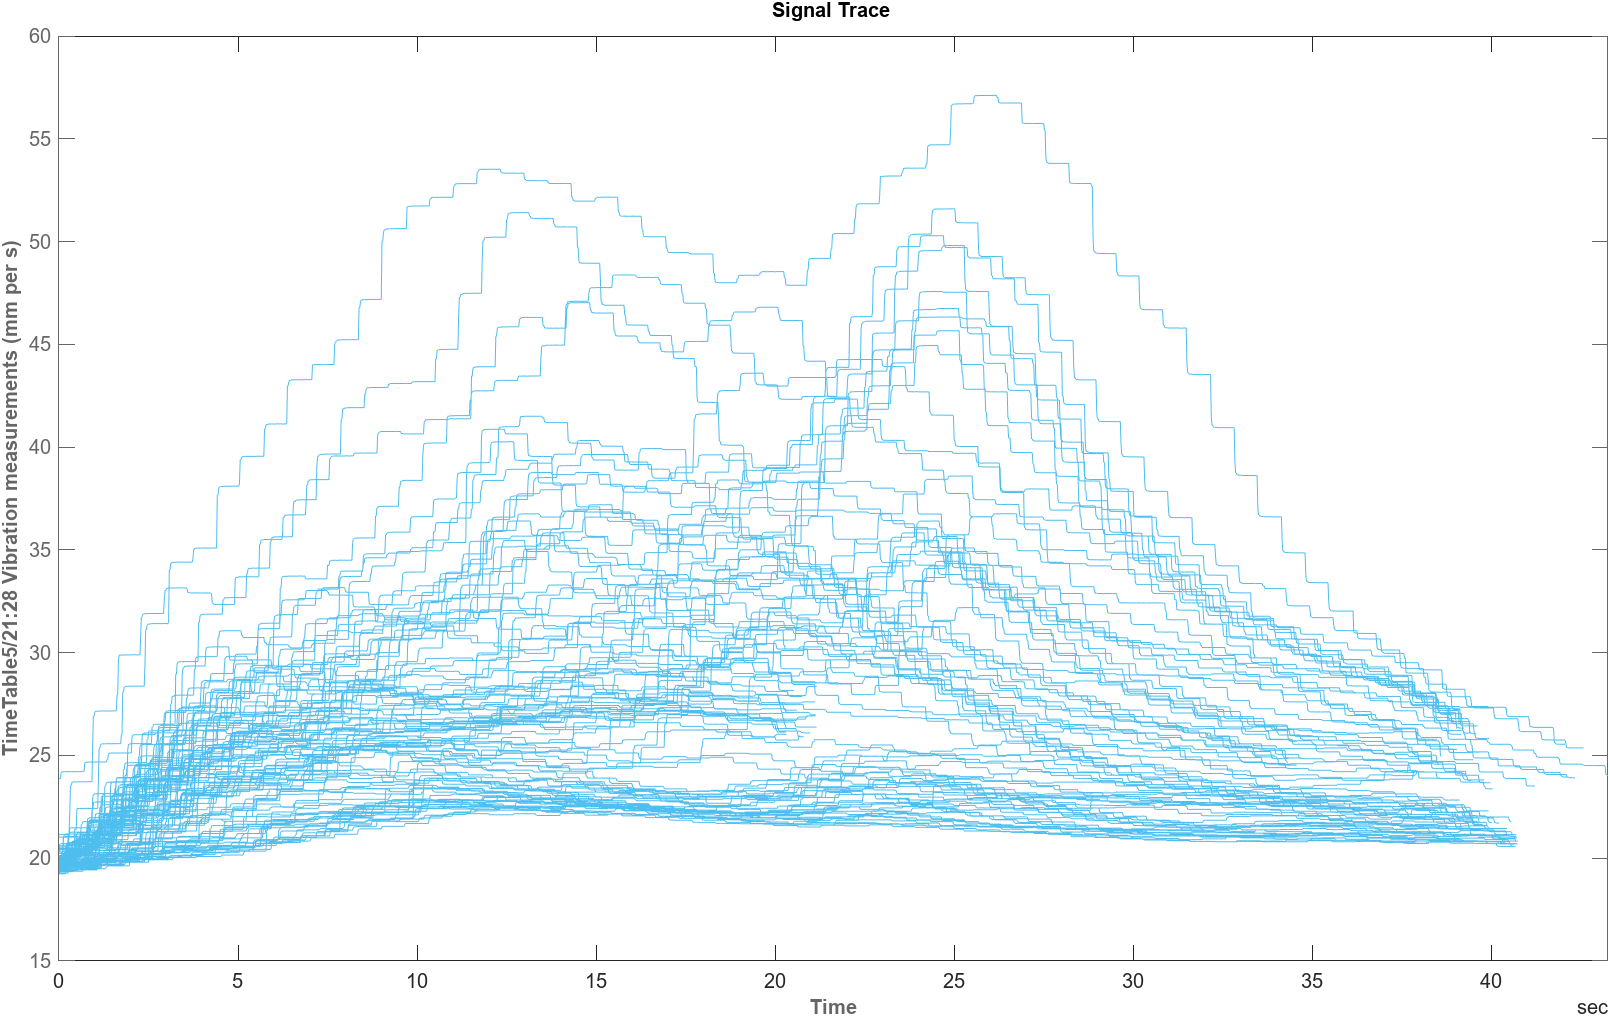
\includegraphics[width=\textwidth, height=\textheight, keepaspectratio]{figures/SignalTrace21.28.png}
    \caption{Signal Trace 21.28}
    \label{fig:SignalTrace21.28}
\end{figure}

Figure \ref{fig:SignalTrace21.07} shows 
\begin{figure}[H]
    \centering
    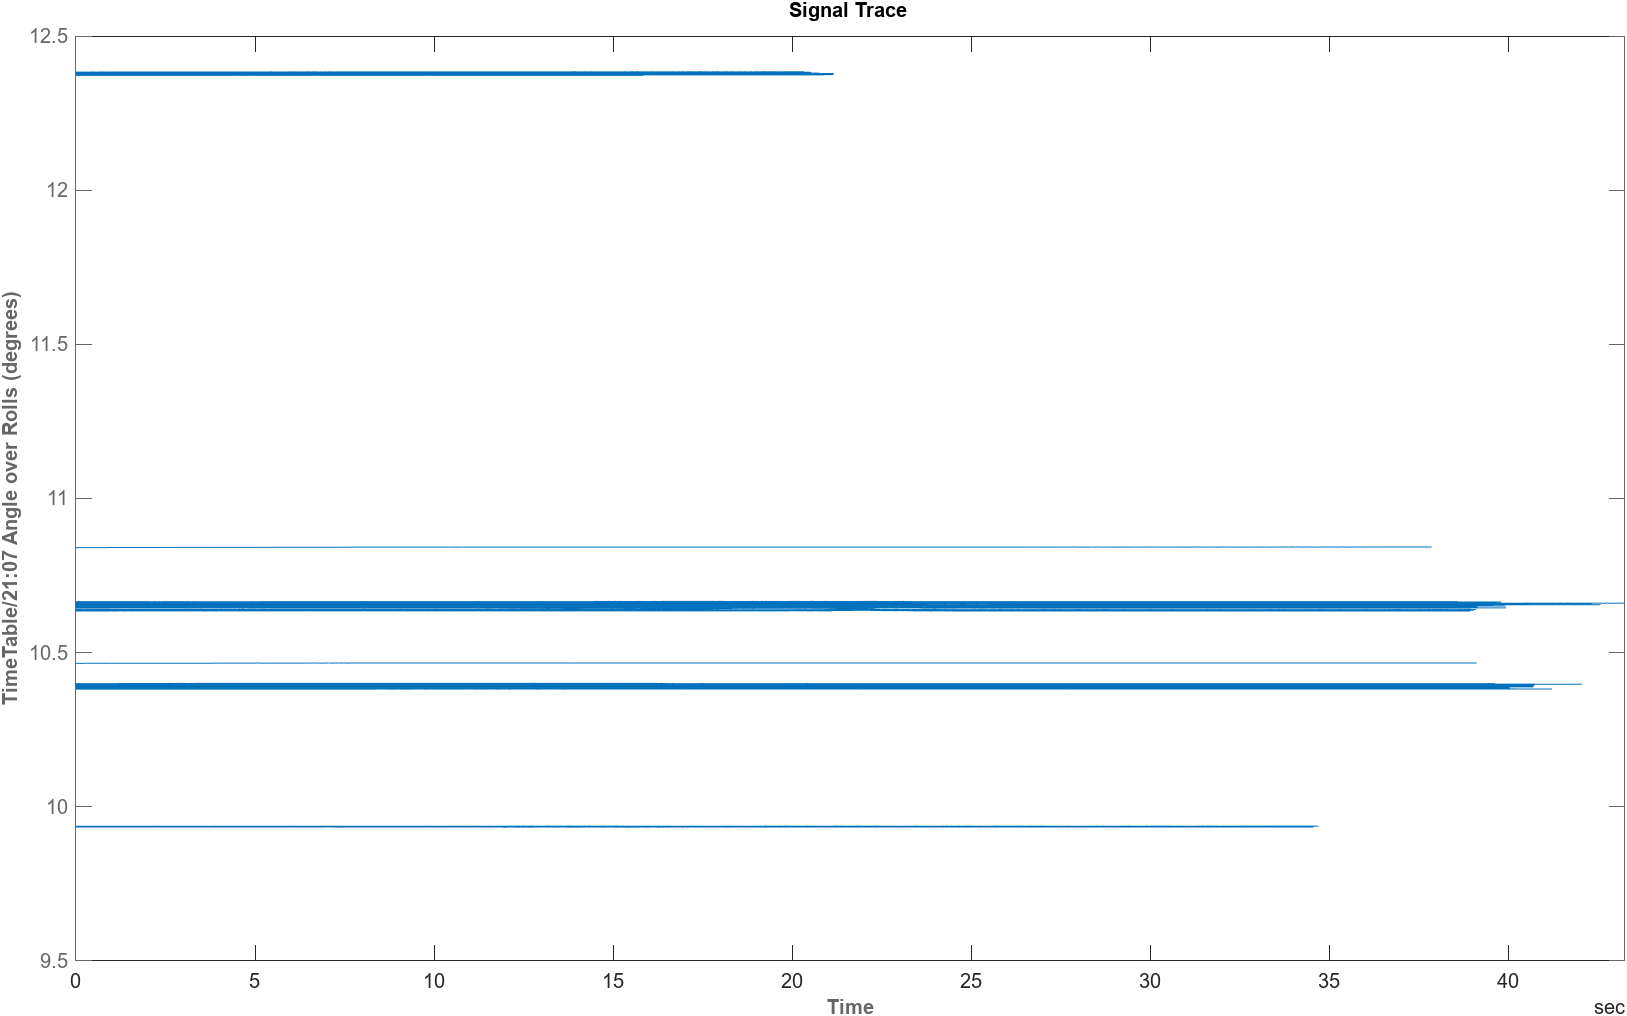
\includegraphics[width=\textwidth, height=\textheight, keepaspectratio]{figures/SignalTrace21.07.png}
    \caption{Signal Trace 21.07}
    \label{fig:SignalTrace21.07}
\end{figure}

Figure \ref{fig:SignalTrace21.35} shows ...
\begin{figure}[H]
    \centering
    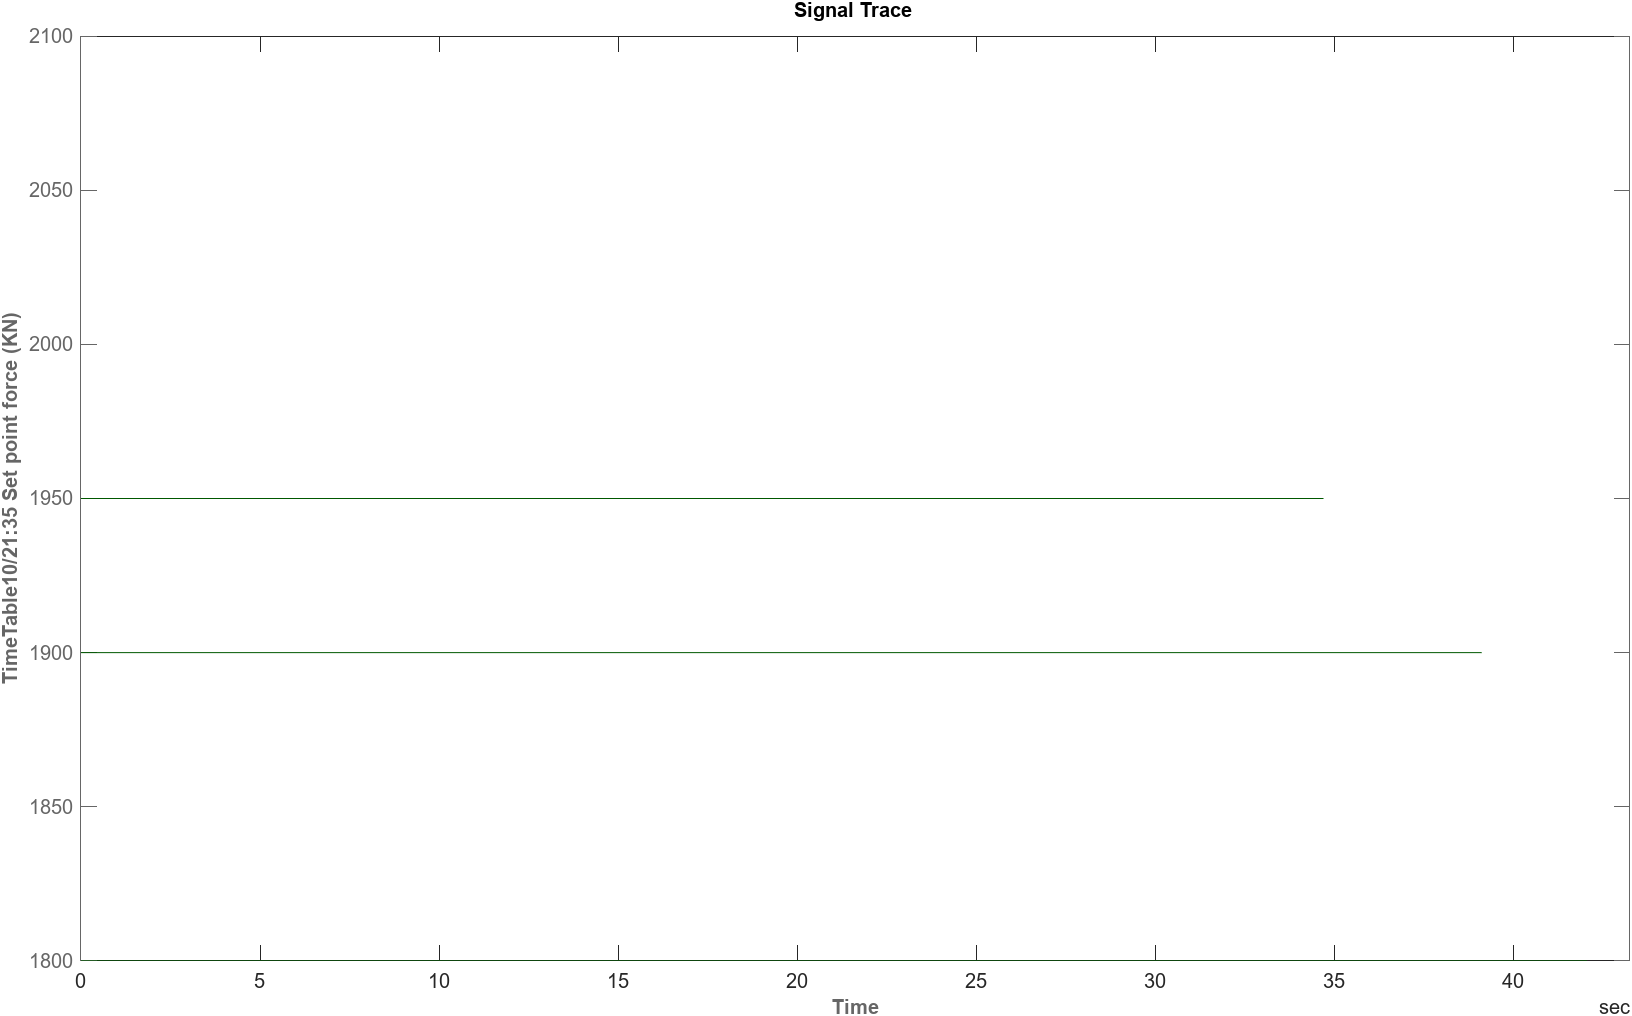
\includegraphics[width=\textwidth, height=\textheight, keepaspectratio]{figures/SignalTrace21.35.png}
    \caption{Signal Trace 21.35}
    \label{fig:SignalTrace21.35}
\end{figure}
\subsection{Coefficient of Determination, R-squared}
\begin{align*}
 R^2 &= 1 - \frac{\textrm{sum squared regression (SSR)}}{\textrm{total sum of squares (SSR)}} \\ 
 &= 1 - \frac{\Sigma(y_i - \hat{y_i})^2}{\Sigma(y_i - \bar{y_i})^2} 
\end{align*}
\subsection{Pre-processing sand State detection}
The state detection for this application is performed using one signal in particular./n
Discuss how many pulses were identified and how many were ruled out by being too short./n
Some of the files contained no pulses at all, B\_30\_03 and B\_04\_04, which means they contribute nothing to this analysis.
Of the remaining 13(?) files 240 pulses were identified using script/function xx./n
When looking at these 240 pulses a number of them are too short and deemed to be false pulses so a threshold of XXs is used to only retain pulses that we think are legitimate pulses.
If we remove the mean from some of the signals we are left with nothing, since some of the signals are straight lines.

Talk about how the data could further classified into different pipe widths.
\subsection{Feature Extraction}
There are a number of features that can be extracted from data 
\subsection{Time Domain Features} 	
Features in the time domain. Statistical features, Impulsive Metrics, 
\subsubsection{Mean}
$$ \bar{x} = \frac{\sum^N_{i=i} x_i}{N} $$
\subsubsection{Standard Deviation}  
$$ Var =\frac{\sum^N_{i=1}(x_i-m)^2}{(N-1)\sigma^2} $$
\subsubsection{Root Mean Square (RMS)}
$$ RMS = \sqrt{\frac{1}{N} \sum^N_{i=1}x^2_i} $$
\subsubsection{Shape Factor}
$$ \frac{ \sqrt{\frac{1}{N} \sum^N_{i=1}x_i^2} }  {\frac{1}{N}\sum^N_{i=1}|x_i|} $$
\subsubsection{Kurtosis} 
$$ Ku = \frac{\sum^N_{i=1}(x_i-m)^4)}{(N-1)\sigma^4} $$ 
\subsubsection{Skewness} 
$$ Sk = \frac{\sum^2_{i=1}(x_i-m)^3}{(N-1)\sigma^3} $$
\subsubsection{Peak Value}
$$ PV = max(x_i) $$ 
\subsubsection{Impulse Factor} 
$$ x_{clear} = \frac{x_p}{(\frac{1}{N}\sum^N_{i=1}|x_i|)} $$  
\subsubsection{Crest Factor} 
$$ CF = \frac{max|x_i|}{\sqrt{\frac{1}{N}}\sum^N_{i=1}x^2_i} $$
\subsubsection{Clearance Factor} 
$$ x_{clear} = \frac{x_p}{(\frac{1}{N}\sum^N_{i=1}\sqrt{|x_i|)^2}} $$
\subsubsection{Signal to Noise Ratio} 
\subsubsection{Signal-to-Noise And Distortion} 
\subsubsection{Total Harmonic Distortion}   
\subsection{Frequency Domain Features}
\subsubsection{Band Power}
\subsubsection{Peak Amplitude}
\subsubsection{Peak Frequency}
\subsection{Models}
\subsubsection{Feature Selection}
\subsubsection{Least Squares Model}
$$ \hat{Y} = (X^T \cdot X) \cdot X^T \cdot y $$
\subsubsection{Metrics}
$$ AIC = 2k - 2Ln(L) $$  
$$ nAIC = log $$
\clearpage  

\section{Results}
Add some plots from the DFD of all pulses and comment on the shape of them all.
Signal 21.07 Angle over Rolls and 21.XX, 21.31, etc are fairly unexciting. They are just straight lines.
Where as signal XX.XX contains a lot of information.
21.35 is a constant signal so when we remove the mean all signals are exactly the same.
Figure \ref{fig:RawSignalCorrelationsFile1}
\subsection{R-squared Correlation}
An analysis of the raw signals was performed using R-squared value. Table \ref{correlationTable} shows the R-squared value for each pair of signals with the lower triangle being a replica of the upper triangle. 
\begin{center}
\begin{tiny}\begin{tabular}{|l|c|c|c|c|c|c|c|c|c|c|c|c|}
\hline
&\textbf{07}&\textbf{10}&\textbf{12}&\textbf{17}&\textbf{20}&\textbf{28}&\textbf{31}&\textbf{32}&\textbf{33}&\textbf{34}&\textbf{35}&\textbf{36}\\\hline
\textbf{07}&1.00&0.00&0.00&0.00&0.00&0.00&0.00&0.00&0.00&0.00&0.00&0.00\\\hline
\textbf{10}&0.93&1.00&0.00&0.00&0.00&0.00&0.00&0.00&0.00&0.00&0.00&0.00\\\hline
\textbf{12}&0.07&0.07&1.00&0.00&0.00&0.00&0.00&0.00&0.00&0.00&0.00&0.00\\\hline
\textbf{17}&0.37&0.44&0.04&1.00&0.00&0.00&0.00&0.00&0.00&0.00&0.00&0.00\\\hline
\textbf{20}&0.07&0.06&0.99&0.03&1.00&0.00&0.00&0.00&0.00&0.00&0.00&0.00\\\hline
\textbf{28}&0.05&0.07&0.88&0.06&0.88&1.00&0.00&0.00&0.00&0.00&0.00&0.00\\\hline
\textbf{31}&0.22&0.26&0.02&0.35&0.02&0.03&1.00&0.00&0.00&0.00&0.00&0.00\\\hline
\textbf{32}&0.20&0.25&0.01&0.32&0.01&0.03&0.99&1.00&0.00&0.00&0.00&0.00\\\hline
\textbf{33}&0.21&0.25&0.01&0.33&0.01&0.03&0.99&1.00&1.00&0.00&0.00&0.00\\\hline
\textbf{34}&0.22&0.26&0.02&0.35&0.02&0.03&1.00&0.99&0.99&1.00&0.00&0.00\\\hline
\textbf{35}&-Inf&-Inf&-Inf&-Inf&-Inf&-Inf&-Inf&-Inf&-Inf&-Inf&-Inf&0.00\\\hline
\textbf{36}&0.16&0.20&0.01&0.26&0.01&0.03&0.77&0.79&0.79&0.77&-0.00&1.00\\\hline
\end{tabular}
\end{tiny}    
\captionof{table}{R2 values for each signal vs. each other signal}
\label{correlationTable}
\end{center}
Figure \ref{fig:RawSignalCorrelationsFile1} is highly linear and from Table \ref{correlationTable} has an R2 correlation value of 0.99. This means that there is not much value to be gained by including both of these signals and likely one can be excluded from analysis.
\begin{figure}[H]
    \centering
    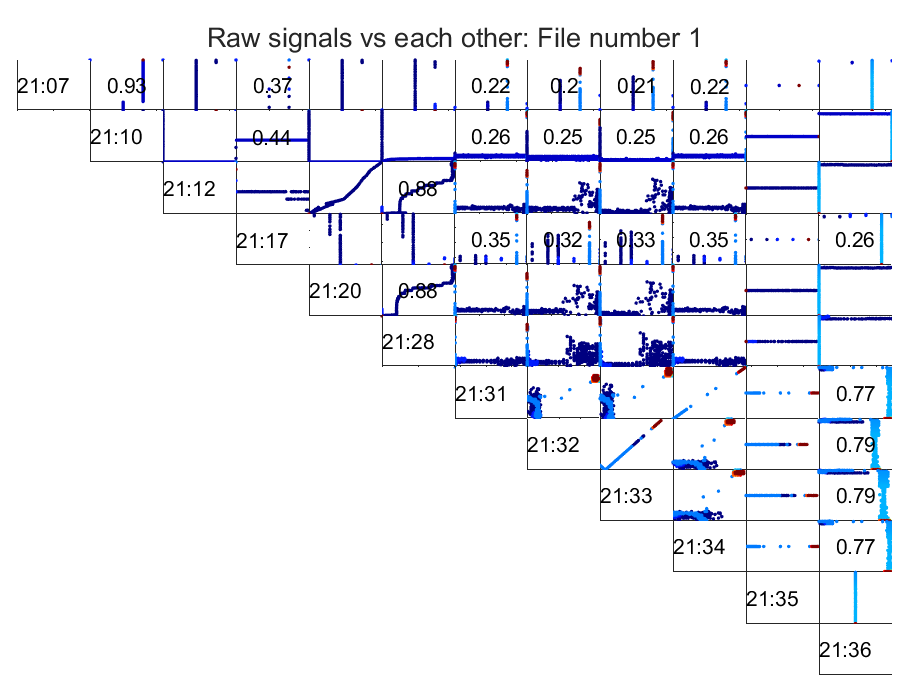
\includegraphics[width=\textwidth, height=\textheight, keepaspectratio]{figures/RawSignalCorrelationsFile1.eps}
    \caption{Plots of each signal vs every other signal R-square values between 0.2 and 0.9 printed on the plot}
    \label{fig:RawSignalCorrelationsFile1}
\end{figure}
Figure \ref{fig:RawSignalCorrelationsFile1} is somewhat linear and from Table \ref{correlationTable} has an R2 correlation value of 0.88.
\begin{figure}[H]
    \centering
    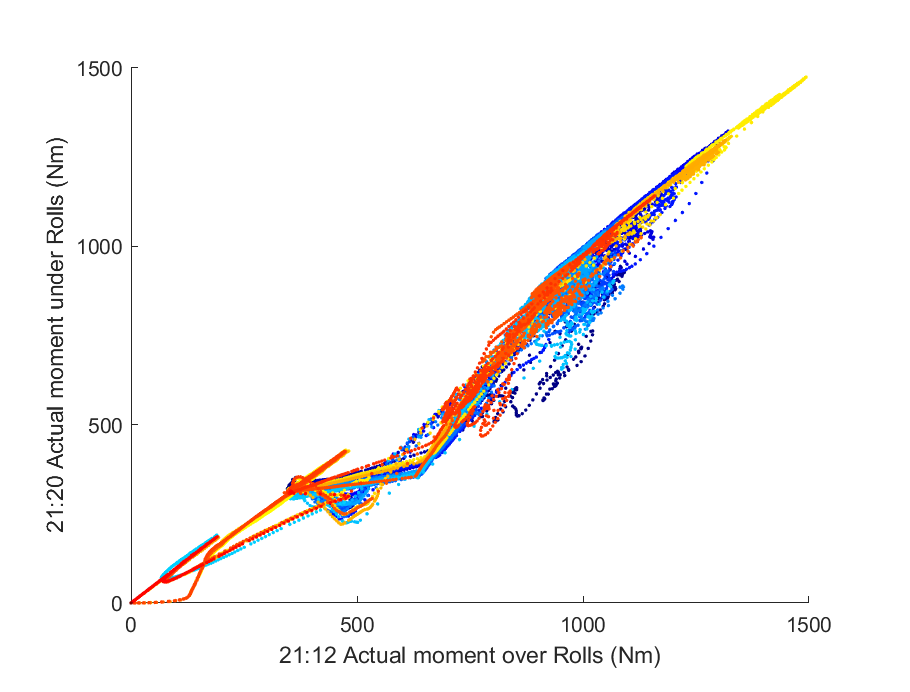
\includegraphics[width=\textwidth, height=\textheight, keepaspectratio]{figures/Signal21_12vSignal21_20.eps}
    \caption{Signal 21.12 vs Signal 21.20}
    \label{fig:Signal21_12vSignal21_20}
\end{figure}	

\begin{figure}[H]
    \centering
    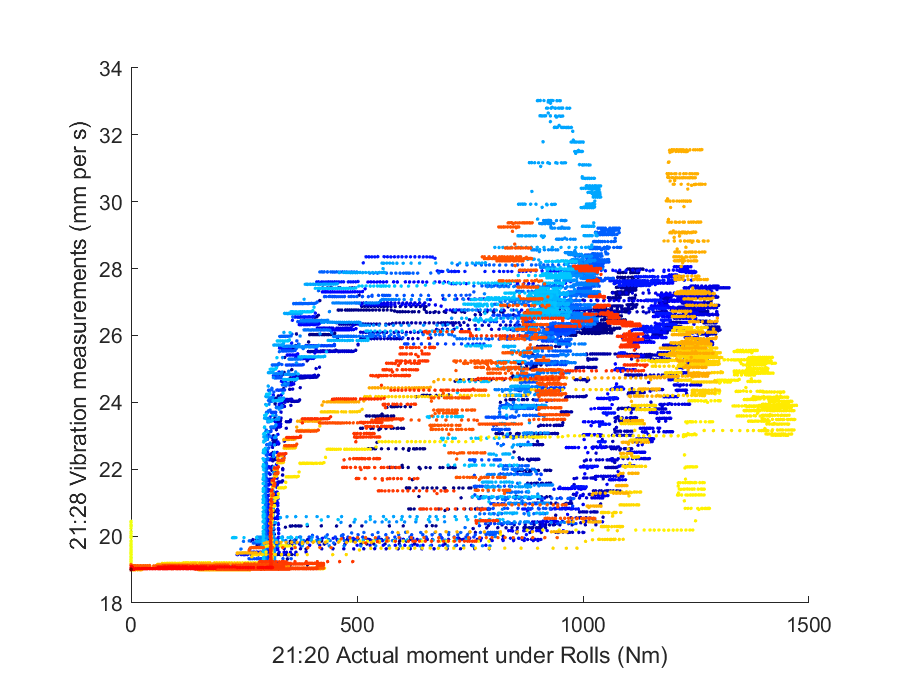
\includegraphics[width=\textwidth, height=\textheight, keepaspectratio]{figures/Signal21_20vSignal21_28.eps}
    \caption{Signal 21.20 vs 21.28}
    \label{fig:Signal21_20vSignal21_28}
\end{figure}	
	
\subsection{Pre-processing}
Figure \ref{fig:StateDetection} shows the windows that were identified from each file where the 21.20 signal was above the threshold. Two files, B\_30\_03 and B\_04\_04, contained no identified pulses. In total 240 pulses were identified. Some of these identified pulses were too short and thus believed to be false positives. Thus any pulse under 500 samples (1 second?) was removed from the data for the next stage leaving 224 pulses to extract features from.

\begin{figure}[H]
    \centering
    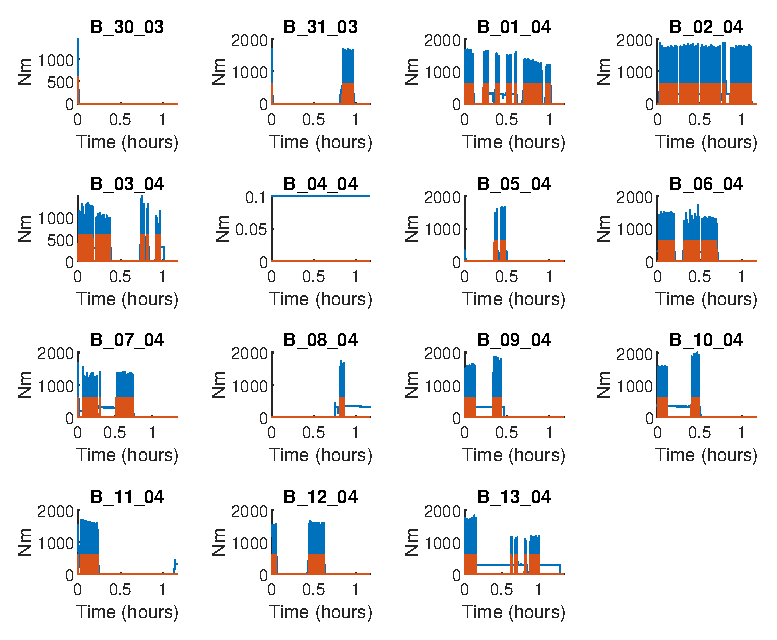
\includegraphics[width=\textwidth, height=\textheight, keepaspectratio]{figures/StateDetectionFig.eps}
    \caption{State detection signal vs 21:20 Actual moment under Rollers}
    \label{fig:StateDetection}
\end{figure}

Figure \ref{fig:StateDetectionFig_B_02_04} shows one of the plots from Figure \ref{fig:StateDetection} in greater detail. This particular file is the one with the highest number of pulses.
\begin{figure}[H]
    \centering
    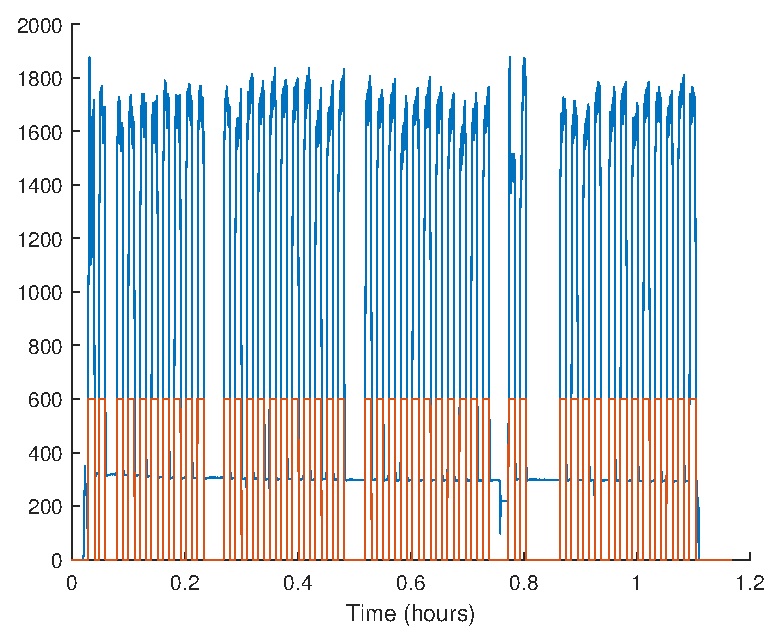
\includegraphics[width=\textwidth, height=\textheight, keepaspectratio]{figures/StateDetectionFig_B_02_04.eps}
    \caption{XXX}
    \label{fig:StateDetectionFig_B_02_04}
\end{figure}

Figure \ref{fig:IdentifiedPulses} show 
\begin{figure}[H]
    \centering
    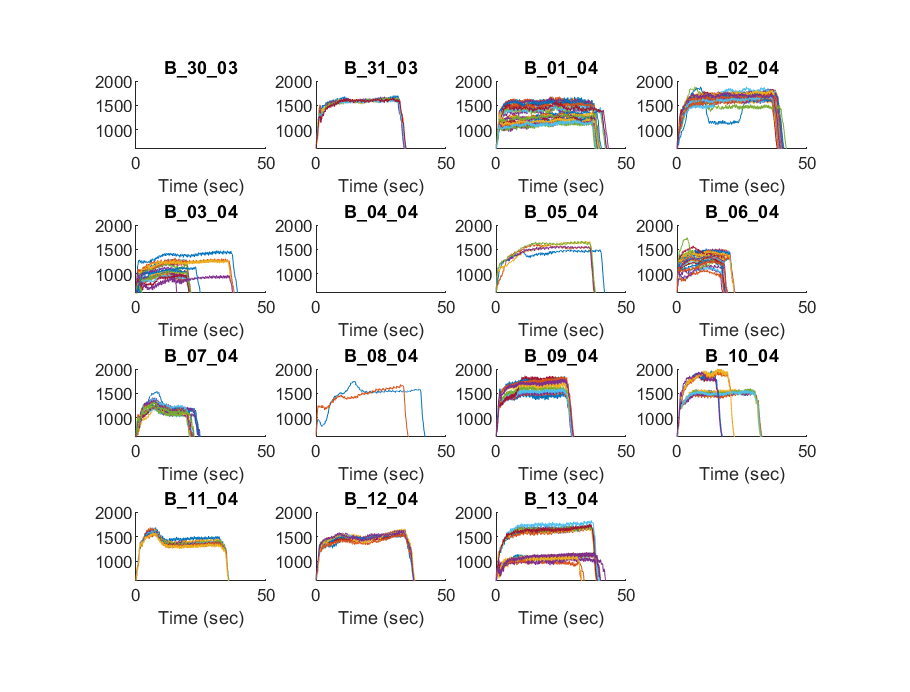
\includegraphics[width=\textwidth, height=\textheight, keepaspectratio]{figures/IdentifiedPulsesFig.eps}
    \caption{Identified pulses in each files for file}
    \label{fig:IdentifiedPulses}
\end{figure}

\subsection{Feature Extraction}
\subsubsection{Feature vs Feature}
Figure \ref{fig:FeatureVsFeatureSignal1} show 
\begin{figure}[H]
    \centering
    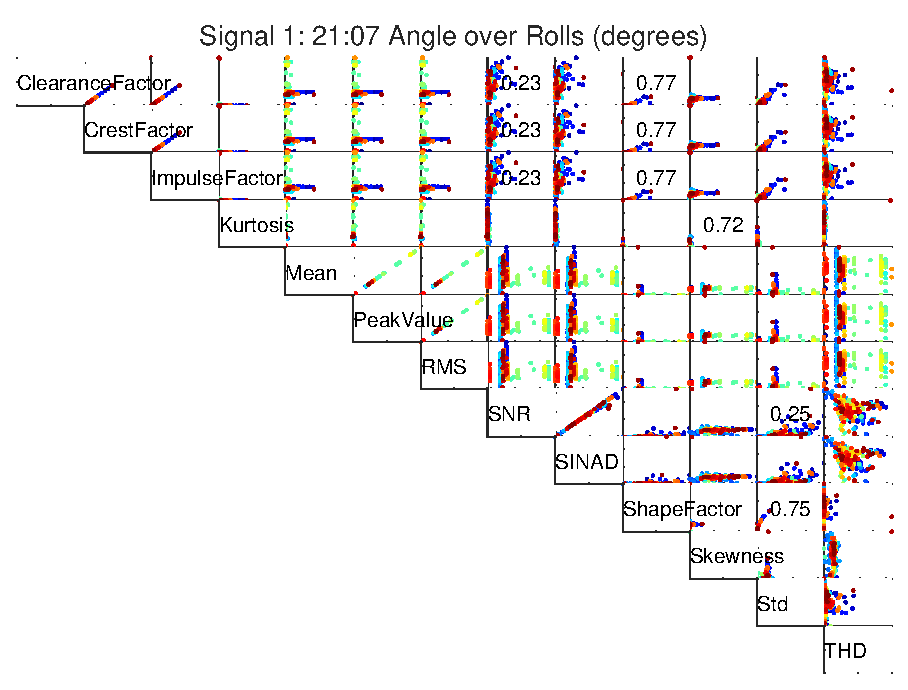
\includegraphics[width=\textwidth, height=\textheight, keepaspectratio]{figures/FeatureVsFeatureSignal1.eps}
    \caption{Feature Vs Feature for Signal 1 21.07}
    \label{fig:FeatureVsFeatureSignal1}
\end{figure}
\subsubsection{Signal vs Signal}
\subsection{Linear models}

\clearpage 
\section{Conclusions}
We are doing inference and not prediction.\\
One conclusion could be that "for future condition monitoring work we need to only focus on this data (might only be 10\%)".\\
Another conclusion could be that we need to go forward to doing this and that.\\
Conclusion could be what we say to the company or what we need.\\
Would temperature of something be good to monitor?\\
Worth doing an analysis based on different sizes
Ideally we would have data over the lifespan of a machine. The data we have right know, we don't know whether is is normal operating data. It could be right at the beginning of the lifecycle or could be just at the end of the machines lifecycle. A system that has been operating for a long period of time will undergo changes due
to the natural wear of the system.
\newpage
\section{Discussion} 
One of the next tasks should be to investigate apply unsupervised learning approaches to the signals highlighted in this project.
\clearpage
\section{References} 
\bibliography{References}
\bibliographystyle{plain} 

\clearpage  
\section{Appendix A - MATLAB Code}

\end{document}